%\begin{document}
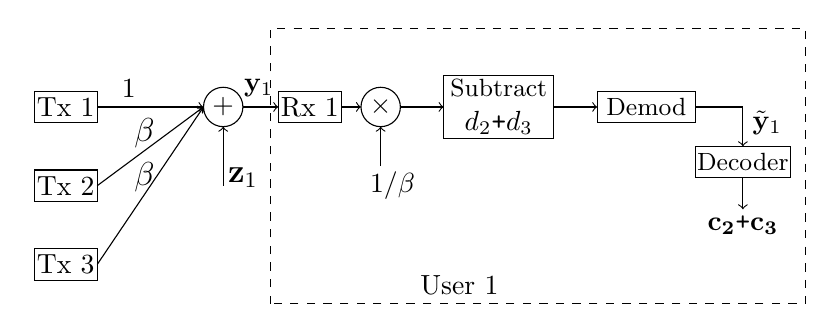
\begin{tikzpicture}

%3 Users
\draw[black] (0.4,0.2) rectangle (-0.4,-0.2); \node at (0,0) {\normalsize Tx 1};
\draw[black] (0.4,-0.8) rectangle (-0.4,-1.2); \node at (0,-1) {\normalsize Tx 2};
\draw[black] (0.4,-1.8) rectangle (-0.4,-2.2); \node at (0,-2) {\normalsize Tx 3};

%Oblique lines to Plus block
\draw [->] (0.4,0) -- (1.75,0); \node [above] at (0.8,0) {1};
\draw [->] (0.4,-1) -- (1.75,0); \node [above] at (1,-0.65) {\large $\beta$};
\draw [->] (0.4,-2) -- (1.75,0); \node [above] at (1,-1.2) {\large $\beta$};


%From + end to Rx1 end
\draw[black] (2,0) circle (0.25); \node at (2,0) {+};
\draw [->] (2,-1) -- (2,-0.25);\node at (2.25,-0.9) {\large $\mathbf{z}_{1}$};

%Receiver 1 block
\draw[black] (2.7,-0.2) rectangle (3.5,0.2); \node at (3.1,0) {\normalsize Rx 1};
\draw [->] (2.25,0) -- (2.7,0);\node[above] at (2.45,0) {\normalsize $\mathbf{y}_{1}$};

%From Rx1 end to 1/beta multiplicator end
\draw[black] (4,0) circle (0.25); \node at (4,0) {$\times$};
\draw [->] (4,-0.75) -- (4,-0.25);\node at (4.15,-1) {\normalsize $1/\beta$};
\draw [->] (3.5,0) -- (3.75,0);

\draw[black] (4.8,0.4) rectangle (6.2,-0.4) node[pos=0.5,align=center] {\small Subtract\\ $d_{2}\texttt{+}d_{3}$}; 
%\node[text width=1.2,align=left] at (5.05,0) {\normalsize Subtract  \\ $d_{2}\texttt{+}d_{3}$};
\draw [->] (4.25,0) -- (4.8,0);

% Input to the Demod
\draw[black] (6.75,0.2) rectangle (8,-0.2) node[pos=0.5,align=center] {\small Demod};
\draw [->] (6.2,0) -- (6.75,0);

%Input to Decoder
\draw [->](8,0) -- (8.6,0) -- (8.6,-0.5);
\node[right] at (8.6,-0.2) {\normalsize $\tilde{\mathbf{y}}_{1}$};
\draw[black] (8,-0.9) rectangle (9.2,-0.5) node[pos=0.5,align=center]  {\small Decoder}; 

%Overview dashed rectangle
\draw [->] (8.6,-0.9) -- (8.6,-1.3);  \node at (8.6,-1.5){\normalsize $\mathbf{c_{2}}\texttt{+}\mathbf{c_{3}}$};
\draw [dashed] (2.6,-2.5) rectangle (9.4,1);\node [above] at (5,-2.5) {\normalsize User 1};

 \end{tikzpicture}
%\end{document} 